\chapter{Calibrated Drift Detection Method} \label{chapt:CDDM}

In this chapter we introduce calibrated drift detection method (CDDM), a drift detection method which detects increases in the irreducible error rate, rather than the overall error rate. Section \ref{CDDM:motivation} motivates the approach to concept drift detection taken by CDDM. Section \ref{cddm:setting} discusses the setting and notation of CDDM. Section \ref{CDDM:algorithm} provides the actual CDDM algorithm. Section \ref{CDDM:limitations} discusses theoretical and practical limitations of CDDM. Section \ref{CDDM:conclusion} summarises this chapter and discusses future work. 

%-------------------------------------------------------------------
% MOTIVATION
%-------------------------------------------------------------------

\section{Motivation} \label{CDDM:motivation}

Most, if not all, extant drift detectors assume that significant increases in the error rate of the base learner are due to concept drift and require model retraining. For example, Gama et al. \cite{DDM} state 
\begin{displayquote}
    Statistical [sic] theory \cite{statistical_theory} guarantees that while the class distribution of the examples is stationary, the error rate of the learning algorithm ($p_i$) will decrease when $i$ increases. A significant increase in the error of the algorithm, suggest a change in the class distribution, and that the actual decision model is not appropriate.
\end{displayquote}

\noindent However, this assumption is invalid in environments when 1) some labels can be predicted more easily than others, and 2) feature drift occurs. Consider the following (fictional) example from our motivating domain of medical triage:
\begin{displayquote}
    At a coronavirus emergency clinic, patients with coronavirus symptoms are being triaged. Young patients have a low mortality rate from coronavirus so are given low priority. Old patients have a high mortality rate so are given high priority. Middle aged patients, however, may have high or low mortality depending on other factors, so may be given a high, low, or medium priority. 
    
    The learner is easily able to discover the relationship between age and priority, but fails to make use of other features. The model thus has a higher error rate for middle aged patients than young or old patients. If there is an increase in the number of middle aged patients with corona virus, then the overall error rate of the model will increase.  
    
    A concept drift detector will may detect the increase in the error rate and signal that the model requires retraining. However, because the actual relationship between instances and labels has not changed, retraining the model would at best be a waste of time, and at worst result in an inferior model trained on a smaller dataset. 
    
    Conversely, suppose that instead of an increase in the middle aged patients there is a {\it decrease in middle aged patients}. This will reduce the average difficulty of the prediction task, and reduce the error rate of the model. 
    
    Suppose that shortly after this occurs, the clinic decides to change its triage policy for dealing with middle aged patients. Because the model is trained to implement the old policy, its error rate for middle aged patients will further increase, but this increase may be cancelled out by the decrease from the reduced number of middle aged patients. 
    
    Thus, a concept drift detector may fail to notice the real drift which has occurred, and the model will not be retrained despite the change in the decision boundary. This situation may therefore result in a false negative.
\end{displayquote}
This example illustrates that a concept drift detector should not monitor for increases in the error rate of the model {\it per se}. Instead it should monitor for increases in rate of {\it reducible} error due to {\it real} drift which is {\it not} predictable {\it ex ante} from the prediction task becoming more difficult on agerage. {\it Virtual} drift which increases the rate of {\it irreducible} error which {\it is} predictable {\it ex ante} is a confounder which can cause false negatives and false positives, such that the model may not be retrained when it should be, and may be retrained when it does not need to be.

%-------------------------------------------------------------------
% SETTING
%-------------------------------------------------------------------

\section{Setting} \label{cddm:setting}

Let $y$ be the true label given to some instance $x$, and $\hat{y}$ be the label predicted by the model. Due to noise, stochasticity, or the limited inferential capabilities of the learner, there is some probability that the model will make the wrong prediction. We thus denote
\begin{equation}
q = \Pr(y=\hat{y})
\end{equation}
as the {\bf reliability} of the model, or the probability that the model will make the correct prediction, for the given instance. 

We assume that the makes probabilistic predictions. We can thus talk about the model {\bf confidence} as the probability assigned by the model to its predicted label, denoted
\begin{equation}
\hat{q} = \hat{\Pr}(y=\hat{y}).
\end{equation}
A plot of a model's confidence versus its reliability is called a {\bf reliability diagram} \cite{calibrating}, and is illustrated in Figure \ref{fig:calibration}. 

\newcommand{\calibrationgraph}[7][]{
    % args:
    \draw [thick, <->] (0,1.25) -- (0,0) -- (1.25,0);
    \node [below] at (1.25,0) {$\hat{q}$};
    14
    \node [left] at (0,1.25) {$q$};
    \node [left] at (0,#7) {$q_t$};
    \node [below] at (#6,0) {$\hat{q}_t$};
    \draw (#2,#3) -- (#4,#5);
    \draw [red] (#6,0) -- (#6,#7);
    \draw [red, dashed] (0,#7) -- (#6,#7);
}

\begin{figure}
    \centering
    \begin{tikzpicture}[scale=3]
        \calibrationgraph{0}{0}{1}{1}{0.5}{0.5}
    \end{tikzpicture}
    \caption{Calibration Graph}
    \label{fig:calibration}
\end{figure}

When a model's confidence is equal to its reliability, $q=\hat{q}$, we say that the model is {\bf calibrated}. So for example, if a calibrated model assigns 0.9 confidence to ten predictions, in expectation one of these predictions will be incorrect. The reliability diagram in Figure \ref{fig:calibration} is of a calibrated model, as it shows an identity relationship between confidence and reliability.

\newcommand{\calibrationgraphB}[7][]{
    % args:
    \draw [thick, <->] (0,1.25) -- (0,0) -- (1.25,0);
    \node [below] at (1.25,0) {$\hat{q}$};
    14
    \node [left] at (0,1.25) {$q$};
    \node [left] at (0,#7) {$Acc$};
    \node [below] at (#6,0) {$\mathbb{E}[\hat{q}]$};
    \draw (#2,#3) -- (#4,#5);
    \draw [red] (#6,0) -- (#6,#7);
    \draw [red, dashed] (0,#7) -- (#6,#7);
}

\newcommand{\virtualdriftgraph}[3][]{
    \begin{tikzpicture}[scale=3]
        \calibrationgraphB{0}{0}{1}{1}{0.5+#2}{0.5+#2}
        \draw [red, thick, ->] (0.5, #3) -- (0.5+#2*1.5, #3);
    \end{tikzpicture}
}

\begin{figure}
    \centering
    \begin{tikzpicture}[scale=3]
        \calibrationgraphB{0}{0}{1}{1}{0.5}{0.5}
    \end{tikzpicture}
        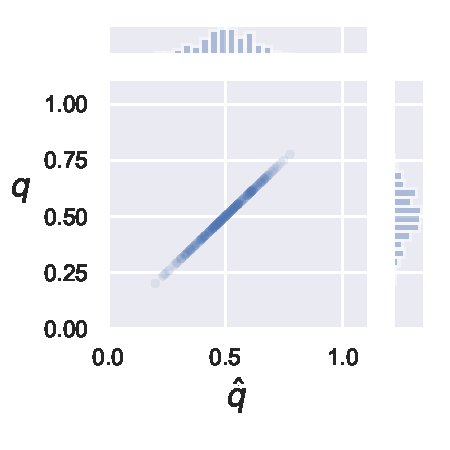
\includegraphics[width=0.3\textwidth]{images/no_drift.pdf}
    \caption{A calibrated model.}
    \label{fig:no_drift}
\end{figure}

When a model is calibrated, we can estimate the accuracy and error rate of the model from its confidence. Figure \ref{fig:no_drift} shows a reliability diagram plus the distribution over confidence values, and thus the distribution over reliability. The accuracy is the expected value of the reliability 
\begin{equation}
    Acc = \mathbb{E}[q]
\end{equation}
and the error rate is one minus the accuracy:
\begin{equation}
    Err = 1 - Acc = \mathbb{E}[q].
\end{equation}
In this manner we may derive an {\it ex ante} estimation of the model's accuracy based on its confidence scores. If the actual {\it ex post} accuracy significantly deviates from this accuracy, then we have evidence that the model is miscalibrated, which we take as evidence of concept drift.

Suppose the average difficulty of the prediction task increases, as described in Section \ref{CDDM:motivation}, and illustrated in Figure \ref{fig:pos_virt}. A calibrated model will decrease in its mean confidence, and our {\it ex  ante} expected error rate will increase. When we observe an {\it ex post} increase in the error rate we will know that this is can be attributed to feature drift rather than due to real drift, and so the model should not be retrained. In other words, we have observed an increase in the irreducible error rather than irreducible error. We can thus avoid false positive.

\begin{figure}
    \centering
    \virtualdriftgraph{-0.2}{0.125}     
    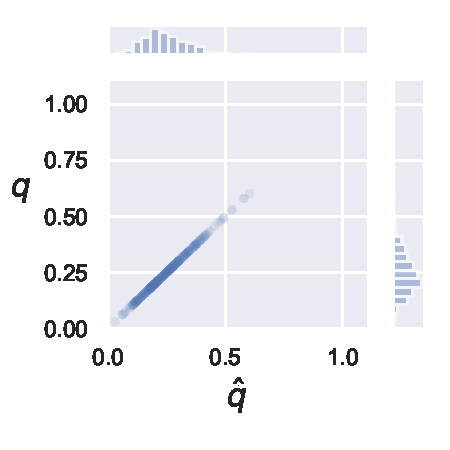
\includegraphics[width=0.3\textwidth]{images/positive_virtual.pdf}
    \label{fig:pos_virt}
    \caption{An increase in irreducible error rate.}
\end{figure}

Conversely, consider the other case described in Section \ref{CDDM:motivation} and illustrated in Figure \ref{fig:co_drift}, where the average difficulty of the prediction task decreases around the same time as real drift occurs. In this case the mean confidence of the model decreases, and so {\it ex ante} error rate decreases. If the {\it ex post} error rate does not decrease, this indicates that concept drift has occurred. In other words, there has been an increase in the reducible error rate, but it has been obscured by a decrease in the irreducible error rate. We can thus detect that the model {\it should} be retrained despite no increase in the overall error rate and thus avoid a false negative.

\begin{figure}
    \centering
    \begin{tikzpicture}[scale=3]
        \calibrationgraphB{0.25}{0}{1}{0.75}{0.75}{0.5}
        \draw [black, thick, ->] (0.9, 0.8) -- (0.9, 0.5);
        \draw [red, thick, ->] (0.6, 0.2) -- (0.85, 0.2);
    \end{tikzpicture}
        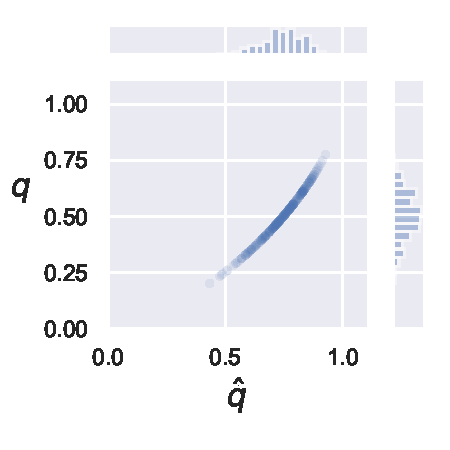
\includegraphics[width=0.3\textwidth]{images/hidden_drift.pdf}
    \caption{A decrease in irreducible error masking an increase in reducible error.}
    \label{fig:co_drift}
\end{figure}

%-------------------------------------------------------------------
% ALGORITHM
%-------------------------------------------------------------------

\section{Algorithm} \label{CDDM:algorithm}

Recall from the Section \ref{background:setting} the following definitions. $y$ is the label which corresponds to a given instance. $\hat{y}$ is the point prediction made by the model for the instance. $q$ is the objective probability of a label given the instance. $\hat{q}$ is the subjective probability assigned to a label by a model.  $\qhatyhat$ is the probability assigned by a model to its preferred prediction $\hat{y}$. 

CDDM approaches the problem of detecting increases in reducible error rather than overall error by estimating irreducible changes in the error rate, and subtracting this from the overall error rate:

Intuitively, CDDM ``places bets" on the label it expects to be correct for each instance. If the model assigns probability $\hat{q}$ to its preferred label, then CDDM buys a bet for \$$\hat{q}$. If the prediction turns out to be correct, CDDM receives a payoff of \$1. If the prediction turns out to be incorrect, CDDM receive a payoff of \$0. If CDDM loses a ``significant" amount of money, then it signals that concept drift has been detected.

Concretely, CDDM obtains residual estimations via calibrated probabilistic predictions. A predictor is {\bf calibrated} if it can assign probabilities to events which match the rates at which these events actually occur \cite{superforecasting}\cite{scoring_rules}\cite{calibrating}. For example, if a calibrated predictor assigns a probability of 90\% to ten events, then in expectation nine of these events should in fact occur. In our notation, a model is calibrated if $q=\hat{q}$. A plot of $q$ against $\hat{q}$ is known as a reliability diagram \cite{calibrating}. Figure \ref{fig:calibration} provides an illustration of the reliability diagram for a calibrated predictor.



How are $\hat{q}$ values to be practically obtained? It is not possible to obtain $\hat{q}$ values for all machine learning techniques. Specifically, this cannot be done for any model which makes only point predictions, and not probabilistic probabilistic predictions. Decision trees are therefore excluded from this discussion. But most popular machine learning techniques produce outputs which can be interpreted as $\hat{q}$ values. For a neural network classifier, the activations of softmax or sigmoid units can be used as $\hat{q}$ values. For ensemble classifiers, the proportions of votes cast for a given label can be interpreted as $\hat{q}$. For a Bayesian model, the posterior probability is naturally interpreted as $\hat{q}$.

Let $\id{y=\hat{y}}=\id{y=0}$, $\qyhat=\Pr(y=0)$, and similarly for $\y{1}$, $\yhat{1}$, $\qhat{1}$, and so on (see Introduction for a full explication of notation). Additionally, let

\begin{align}
    \qyhat &= \Pr(y=\hat{y}) \\
    \qhatyhat &= \max(\qhat{0},\qhat{1})
\end{align}
These indicate the probability of the model making a correct prediction, and the models own estimation of this probability, respectively. 

CDDM takes as a null hypothesis that the base learner is calibrated. That is, the area in Equation \ref{eq:calibration_area} is equal to zero. In this case we have
\begin{align}
	\mathbb{E}\left[ \qhatyhat - \id{y=\hat{y}}  \right] &= \qyhat \cdot (\qhatyhat - 1) + (1-\qyhat) \cdot (\qhatyhat-0) \\
    &= \qyhat\qhatyhat - \qyhat + \qhatyhat - \qyhat\qhatyhat \\
    &= \qhatyhat - \qyhat.\label{eq:expectation}
\end{align}

Using this expected value, we can bound the probability of $\qhatyhat_t$ and $\id{y=\hat{y}}_t$ values to accumulating to a value as extreme as $k$ at time $T$
\begin{align}
    P\left(  \sum_{t=1}^T \frac{\qhatyhat_t - \id{y=\hat{y}}_t}{T} \ge k \right)
    &\le \exp\left(-\frac{2T^2k^2}{\sum_{t=1}^t(b_t - a_t)^2}\right) \\
    \intertext{Where $a_t$ and $b_t$ are lower and upper bounds on $\qhatyhat_t-\id{y=\hat{y}}_t$, respectively. Because $0\le \qhatyhat_t, \id{y=\hat{y}}_t\le 1$, we have that $a_t=-1 \le \qhatyhat_t-\id{y=\hat{y}}_t \le b_t=1$, so the right side of the inequality simplifies to}
  &\le \exp\left(-\frac{2T^2k_T^2}{\sum_{\tau=1}^t 4}\right) \\
  &\le \exp\left(-\frac{Tk_T^2}{2}\right). \label{eq:hoeffding}
\end{align}
This equation gives us a $p$-value of for an observed sequence of $\id{y=\hat{y}}$ and $\qhatyhat$ under the null hypothesis of calibration. If this value falls below some critical threshold, we may reject the null hypothesis and conclude that the model is uncalibrated. 

Similar to several other drift detectors \cite{DDM}\cite{HDDM}\cite{FLORA}, we use two critical thresholds: $\alpha_{warn}$, a warning threshold, and $\alpha_{drift}$, a drift threshold. When $P$ falls below $\alpha_{warn}$ for any $T$ value, CDDM issues a warning that drift may be occurring. When $P$ falls below $\alpha_{warn}$ for any $T$, CDDM signals that drift has been detected, and the referral documents since the earliest $T$ for which $P<\alpha_{warn}$ can be retrieved to retrain the model. We use the values $\alpha_{warn}=0.05$ and $\alpha_{drift}=0.01$.

Equation \ref{eq:hoeffding} indicates a trade-off in our choice of $T$, which in the streaming context denotes how large is the window of recent examples we are testing for miscalibration. The bound shrinks as $T$ and $k_T$ increase. However, if $T$ is large, then $k_T$, the mean value of $\qhatyhat-\id{y=\hat{y}}$ will be diluted by many pre-miscalibration instances. We do not have a principled way to choose a good value of $T$. Instead we propose maintaining a sliding window of $N$ values of $\qhatyhat-\id{y=\hat{y}}$, and testing the most recent $T$ instances for $T=1,2,\dots,N$. This introduces multiple comparisons and requires making a Bonferonni correction to our drift and warning bounds. The full pseudocode is given in Algorithm \ref{alg:cddm_basic}.

\begin{algorithm}
    \caption{CDDM}
    \label{alg:cddm_basic}
    \begin{algorithmic}
        \Require Warning threshold $\alpha_{warn}$
        \Require Drift threshold $\alpha_{drift}$
        \Require Window size $N$
        \State Window $\gets$ []
	\For {$y_t, \qyhat_t, \hat{y}_t$ in the data stream}
%            \State $\qhatyhat \gets \max(\qyhat,1-\qyhat)$
            \State Window.pop()
	    \State Window $\gets (\id{y=\hat{y}} - \qhatyhat) \cup$ Window
            \For {$T=1,2,\dots,N$}
                \State Calculate $p$ value for Window[:T]
                \If {$p \leq \alpha_{drift}/2N$}
                    \State {\tt status} $\gets$ {\tt drift}
                \ElsIf {$p_{min} \leq \alpha_{warn}/2N$}
                    \State {\tt status} $\gets$ {\tt warn}
                \EndIf
            \EndFor
        \EndFor
    \end{algorithmic}
\end{algorithm}

%-------------------------------------------------------------------
% LIMITATIONS
%-------------------------------------------------------------------

\section{Limitations} \label{CDDM:limitations}

\subsection{Theoretical Limitations}

There remains the possibility of miscalibration being undetectable by monitoring the area described in Equation \ref{eq:calibration_area} under certain conditions. One such condition is illustrated in Figure \ref{fig:weird_calibration}. It is not clear when such a situation could arise, and indeed if such a situation is even plausible. Further work is required to resolve this issue.

\begin{figure}
    \centering
    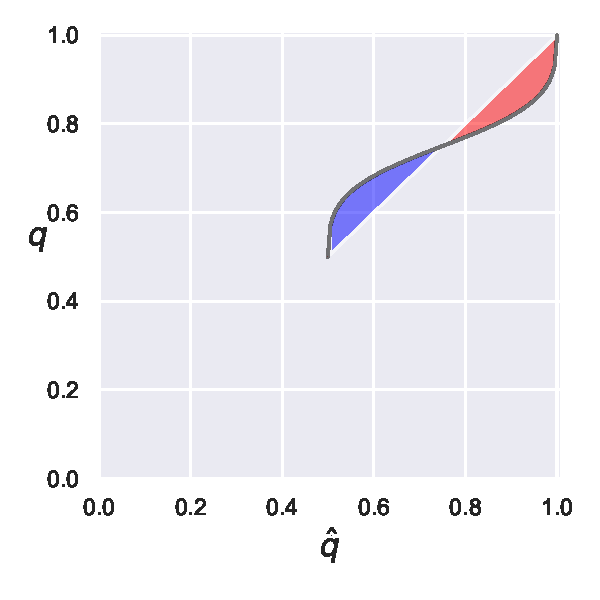
\includegraphics[width=0.5\textwidth]{images/cddm_area2.pdf}
    \caption{Example of a miscalibration undetectable by CDDM.}
    \label{fig:weird_calibration}
\end{figure}

We now consider the question of choosing an appropriate window size $N$. Given a window size $N$, our drift detection threshold will be given by $\epsilon/N$. Suppose also, that for the most recent $n$ examples we have had $\hat{q}-q=\delta$. That is, the model has become overconfident by $\delta$. Then the p-value will be given by
\begin{equation}
    \exp\left(-\frac{n^2\delta^2}{2N}\right)
\end{equation}
setting this equal to the threshold will give us the minimum time under the new distribution until the miscalibration can be detected. This gives
\begin{align}
    \exp\left(-\frac{n^2\delta^2}{2N}\right) &= \frac{\epsilon}{N} \\
    \delta &= \sqrt{-\frac{2N}{n^2}\ln\left(\frac{\epsilon}{N}\right)}
\end{align}
We get minimum $\delta$ when $n=N$. In this case, it takes the entire window to full up for the drift to be detected. Thus, the range of detectable $\delta$ given a window size $N$ is
\begin{equation}
    1 \ge \delta \ge \sqrt{-\frac{2}{N}\ln\left(\frac{\epsilon}{N}\right)} \label{eq:window_size}
\end{equation}

Figure \ref{fig:cddm_window_size} illustrates the minimum detectable $\delta$ against $N$ (black line), as well as the time to detect miscalibrations of $\delta$ values for a range of $N$ values (dashed lines).

\begin{figure}
    \centering
    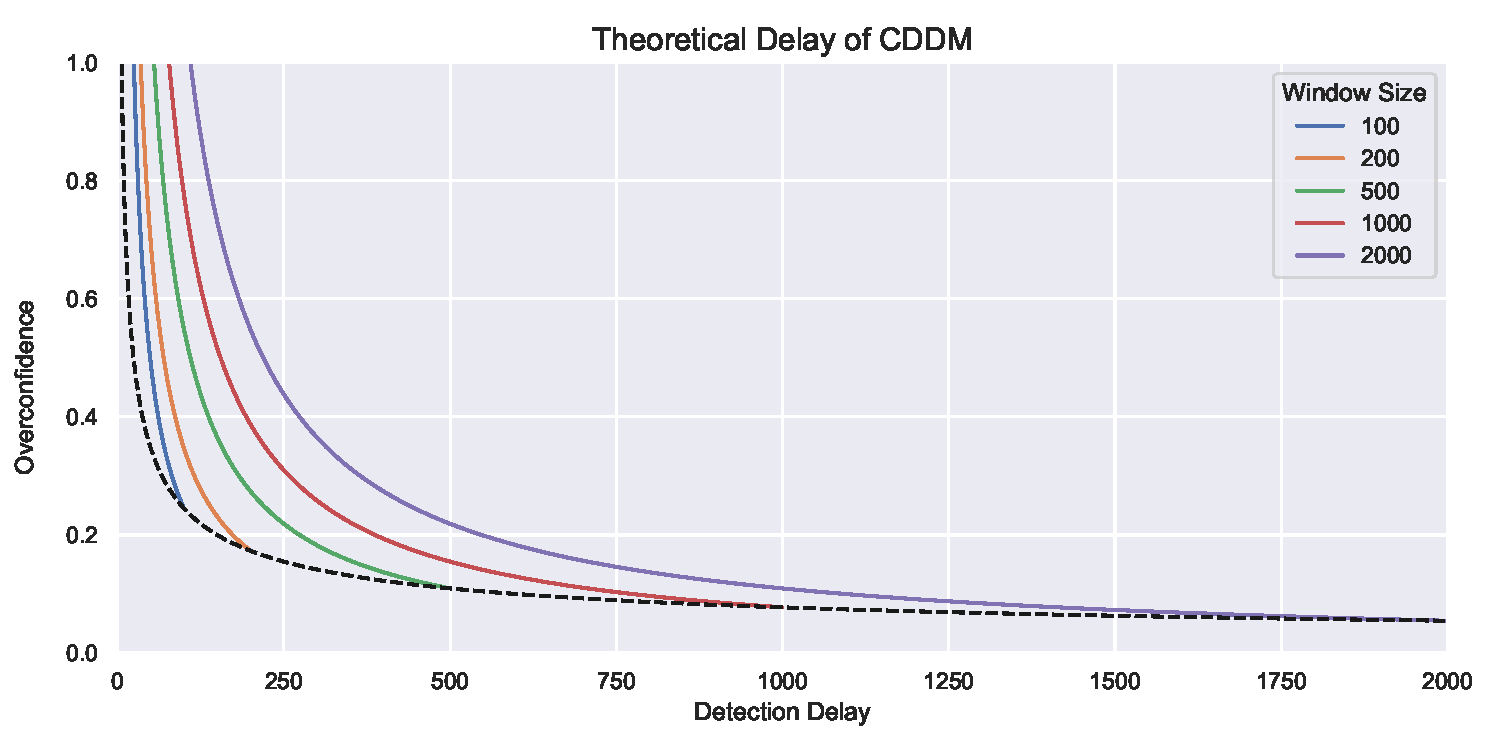
\includegraphics[width=\textwidth]{images/cddm_window_size.pdf}
    \caption{Detection delay (x-axis) vs $\delta$ (y-axis). The black line gives the minimum detectable $\delta$ for a window size $x$. The dashed lines are detection delays for window sizes of (from left to right) 100, 200, 500, 1000 and 2000.}
    \label{fig:cddm_window_size}
\end{figure}

An appropriate choice for window size $N$ can therefore be obtained by 1) if there is a smallest miscalibration degree $\delta$ which {\it requires} being detected, then one can obtain the appropriate window size using Equation \ref{eq:window_size}. 2) Otherwise, one may consult Figure \ref{fig:cddm_window_size}, and choose a window size which is appropriately reactive to miscalibration for the target domain.

%-------------------------------------------------------------------
% CALIBRATION
%-------------------------------------------------------------------

\subsection{Calibration}

The second main limitation of CDDM is that it takes as axiomatic that its base learner is calibrated, when in fact few machine learning models are actually calibrated unless measures are taken to ensure this.



\cite{nn_calibration}
\cite{trust_model_uncertainty}

If a predictor over-estimates the probabilities of a target outcome (in our case, a correct classification), and $\hat{q}>q$, then the model is {\bf overconfident}. Overconfident models can be considered as ``pushing" values towards 1 in the mapping from $q$ to $\hat{q}$.
\item Conversely, if a predictor under-estimates the probabilities of a target outcome, and $\hat{q}<q$, then the predictor is {\bf underconfident}. Underconfident models can be considered as pushing $q$ values towards 0.

If a predictor is overconfident close to 1 and underconfident close to 0, then the predictor is {\bf extremist}. Extremist models can be considered as pushing $q$ values towards 0 {\it and} 1. Maximum margin methods such as boosted trees and boosted stumps are prone to extremism \cite{calibrating}. Often an extremist predictor can be calibrated by applying a sigmoid-shaped map to subjective probabilities.

The opposite type to extremisim is {\bf moderatism}, in which the predictor is underconfident close to 1 and overconfident close to 0. Thus, $q$ values are pushed {\it away from} 0 and 1. Na\"{i}ve Bayes models are prone to moderatism due to making unrealistic independence assumptions \cite{calibrating}. 

The terms ``overconfident" and ``underconfident" come from Tetlock \cite{superforecasting}. ``Extermism" and ``moderatism" are our own terminology. These relationships are illustrated with reliability diagrams in Figure \ref{fig:calib_drift_types}. Note that this list not exhaustive. Any function $f:[0,1]\rightarrow[0,1]$ is a possible relationship between $q$ and $\hat{q}$ for some model.

\begin{figure}%[t!]
    \centering
    \subfigure[Underconfident]{
        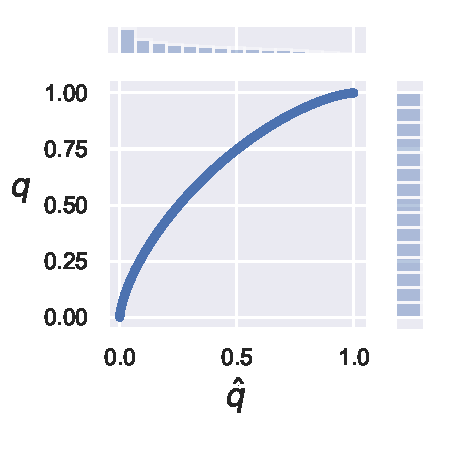
\includegraphics[width=0.45\textwidth]{images/overconfident.pdf}
    }
    \subfigure[Overconfident]{
        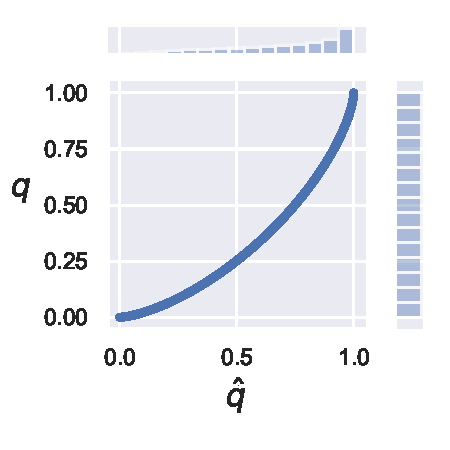
\includegraphics[width=0.45\textwidth]{images/underconfident.pdf}
    }
    \subfigure[Extremist]{
        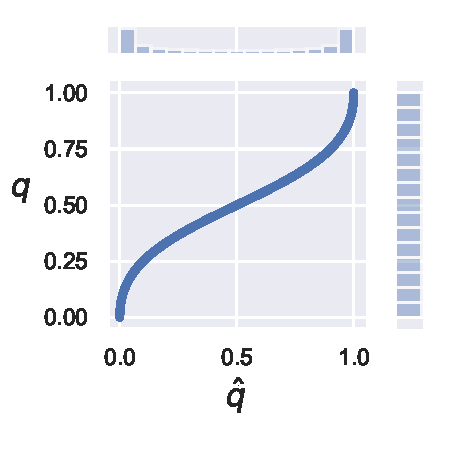
\includegraphics[width=0.45\textwidth]{images/extremist.pdf}
    }
    \subfigure[Moderate]{
        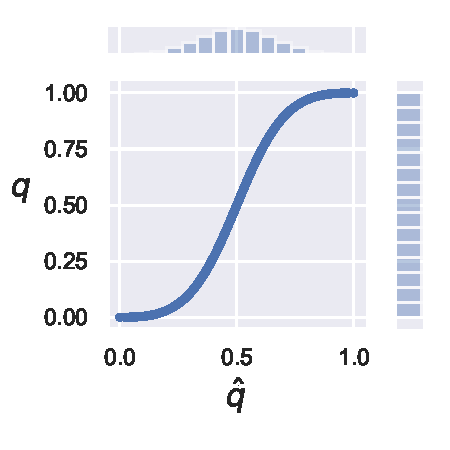
\includegraphics[width=0.45\textwidth]{images/moderate.pdf}
    }
    \caption{Reliability diagrams for a few relationships between $q$ and $\hat{q}$.}
    \label{fig:calib_drift_types}
\end{figure}

With the vocabulary of calibration and reliability diagrams, we may now return to our problem as laid out in Section \ref{CDDM:motivation}. We wished to derive an algorithm which could detect real drift {\it separately} from feature drift, as it it is only real drift which results in a change in the decision boundary. 

We identified two failure modes of only monitoring for increases in the error rate as a means of detecting concept drift. First, feature drift may trigger a drift detection, due to the average difficulty of the classification tasks increasing. Second, if feature drift and real drift co-occur, then the detector may fail to notice the concept drift due to the average difficulty of the classification tasks decreasing. 

These scenarios can be neatly expressed with reliability diagrams. Figure \ref{fig:no_drift} shows an initial distribution of data. The model is calibrated, and the $\hat{q}$ values centre around 0.5. These two facts together tell us that $\Pr(y=\hat{y})\approx 0.5$. 

Figure \ref{fig:co_drift} depicts the scenario in which real and feature drift co-occur, and the latter hides the former. A model in this situation would benefit from retraining, and yet a drift detector which is monitoring the error rate will not be triggered. Figure \ref{fig:pos_virt} depicts the scenario in which feature drift triggers will trigger a drift detector, despite no change in the decision boundary.



What we have shown by these examples is that concept drift detectors should not be monitoring for changes in the error rate, as this influenced by feature drift, and will lead to impaired performance. Instead, we should be monitoring for changes in the reliability diagram of a model. This is the true test for whether real drift has occurred, regardless of what feature drift may or may not be occurring.


\subsection{Calibration Maps}

If a model was not trained using a proper scoring rule, or for some other reason is not well calibrated, then it can become approximately well-calibrated using a {\bf calibration map}. There are several approaches to producing calibration maps, described below.

Logistic calibration - also called {\bf Platt scaling} \cite{platt} - calibrates model predictions by passing them through a parametric calibration map, specifically a sigmoid function. If $\bar{p}$ is the (uncalibrated) model output, then a calibrated probability is given by
\begin{equation}
	p = \frac{1}{1 + \exp(a\bar{p} + b)}
\end{equation}
where the parameters a and b are fitted using maximum likelihood estimation on a calibration set $(p_1,L_1),\dots,(p_n,L_n)$. Note that this calibration set must be distinct from the training set, but can be the same set as used for (hyper)parameter selection. Specifically, $a$ and $b$ are derived from performing gradient descent on the loss function
\begin{equation}
	- \sum_i L_i \log( p_i ) + (1-L_i) \log(1-p_i)
\end{equation}
To avoid overfitting, Platt recommends modifying the loss values before fitting the sigmoid calibration map as follows:
\begin{equation}
	L_i' = \begin{cases}
		\frac{N_1 + 1}{N_1 + 2} & \text{if }L_i=1 \\
		\frac{1}{N_0 + 2} & \text{if }L_i=0 \\
	\end{cases}
\end{equation} 
where $N_0$ is the number of zero-valued losses, and $N_1$ is the number of one-valued losses. 

Isotonic calibration is a non-parametric method of producing calibration maps \cite{isotonic_calibration}. It follows that it is more flexible than logistic calibration, but also more prone to overfitting. The only assumption isotonic regression makes about the reliability diagram is that it is isotonic, that is, it is monotonically increasing. 

Beta calibration is another parametric calibration map family \cite{beyond_sigmoids}. It takes the form
\begin{equation}
	p = \frac{1}{1 + 1/\left(e^c\frac{\hat{p}^a}{(1-\hat{p})^b}\right) }
\end{equation}
where $a,b\ge 0$ so that the map is monotonically non-decreasing. This map can be fitted as easily as a logistic map \cite{beyond_sigmoids}.

Beta calibration is intended to overcome some of the drawbacks of logistic calibration. Logistic calibration results in distortions for many classifiers including Naive Bayes and Adaboost which can result in worse probability estimates than the original. The  strength of logistic calibration is that it tends towards producing exactly correct calibration when a model's uncalibrated probabilities are normally distributed. Beta calibration, on the other hand, tends towards correct calibration when the uncalibrated probabilities are beta distributed.

Experiments have found beta calibration to be superior to logistic calibration for Na\"{i}ve Bayes, Adaboost, Random Forest, logistic regression, SVM, and MLP \cite{beyond_sigmoids}. 

%-------------------------------------------------------------------
% CONCLUSION
%-------------------------------------------------------------------

\section{Conclusion} \label{CDDM:conclusion}

In this chapter we introduced calibrated drift detection method (CDDM). We argued that a drift detector should detect increases in the reducible error rate rather than the overall error rate, so as to avoid unnecessary retraining. CDDM takes this approach to concept drift detection by detecting when a model becomes uncalibrated. However, CDDM still has some significant limitations. Theoretically, CDDM can only detect mean overconfidence below a certain level determined by the window length. Practically, CDDM assumes that a learner is initially calibrated, whereas most models are not natively calibrated and post-hoc calibration techniques have significant limitations.

A promising direction for future work would be building a calibration map online, and detecting when this calibration map changes, rather than assuming the learner is calibrated in the first place.